\section{Uppgift 3}\label{sec:uppg03}

\subsection{Instruktioner}
\begin{verbatim}
3. Skriv ett program som räknar ut vilket av tre heltal som är det mellersta
   talet och sedan skriver ut detta tal. Användaren ska skriva in det tre
   heltalen, exempel på utskrift:

        Skriv in första talet: *7*
        Skriv in andra talet: *10*
        Skriv in tredje talet: *4*
        Det mellersta talet är 7
\end{verbatim}

\subsection{Lösning}
För att hitta medianen av en uppsättning tal;
Sortera talen efter värde, medianen är i listans mellersta position.
Enligt wikipedia 
I algoritmstudier är ett välbekant problem att hitta medianen bland fem tal med
endast sex jämförelser.

%   [ A ]    [ B ]    [ C ]
%
%   Vilket av talen A, B och C är det mellersta?
%
% A större än B ?
%       B större än C ?
%               SVARET ÄR B         [ A ]    [ B ]    [ C ]
%       A större än C ?
%               SVARET ÄR C         [ B ]    [ C ]    [ A ]
%       Annars
%               SVARET ÄR A         [ B ]    [ A ]    [ C ]
% Annars
%       A större än C ?
%               SVARET ÄR A         [ C ]    [ A ]    [ B ]
%       B större än C ?
%               SVARET ÄR C         [ A ]    [ C ]    [ B ]
%       Annars
%               SVARET ÄR B         [ A ]    [ B ]    [ C ]
%
\subsubsection{Funktion}
% TODO: Eventuell beskrivning av #03 funktionalitet.

\subsubsection{Kommentar}
% TODO: Eventuell kommentar på #03.


\subsubsection{Källkod}
\inputminted[linenos]{java}{src/Lab2Uppg03.java}
\caption{Lab2Uppg03.java}
\label{src:uppg03}
% TODO: Lägg till källkod för #03.


\subsubsection{Skärmdump}
\begin{figure}[htbp]
    \centering
        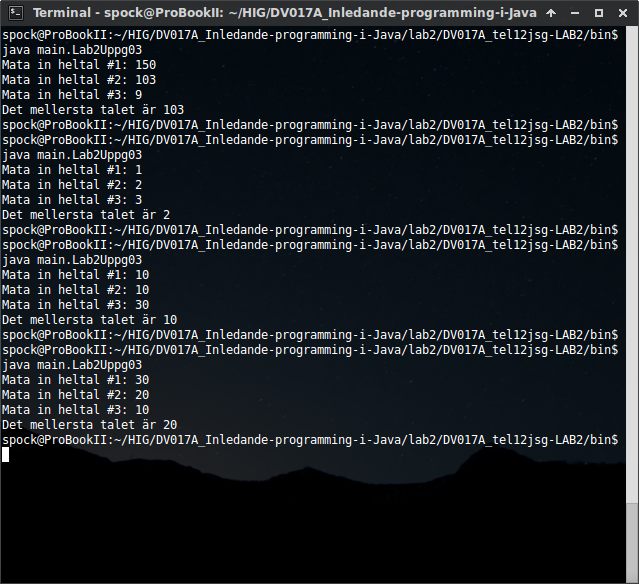
\includegraphics[width=\linewidth]{img/03.png}
    \caption{Körning av koden till Uppgift \ref{sec:uppg03}}
    \label{fig:uppg03-screenshot}
\end{figure}
% TODO: Lägg till skärmdump av #03.

